%\newpage

\section{Design of different barriers}
\label{design}

In this section we summarize different designs for barrier
implementation and their characteristics. Based on the discussion presented
in the previous section, we try to reduce the overhead of a barrier
by decreasing the contention for a shared memory location
and reducing the volume of data transmitted on the network.
We start with a simple barrier implementation using \emph{Fetch-and-Add}.

\subsection{Barrier with Fetch-and-Add}
\label{sec:fetchandadd}

In this case, a global counter is allocated in the shared memory of a
parallel system. Before a barrier starts, the counter will be set to
the number of threads participating in the parallel region. As the
threads come to the barrier point, each one will decrease the counter
with an atomic fetch-and-add operation and then spin on
checking the counter value until the result is zero.

This implementation is quite similar to the barrier implementation
introduced in
\cite{IBM92}. The difference is that instead of doing scheduling, a
busy-wait method is enforced by letting each thread constantly read
the shared counter. The whole process is shown in Figure
\ref{fig:fetchandadd}. 

In the diagram, we use square blocks to represent our data structure,
and arrowed lines with comments to represent actions that a thread may
apply to the structure, in this case, the shared memory counter.

\begin{figure*}[htbp]
  \begin{center}
    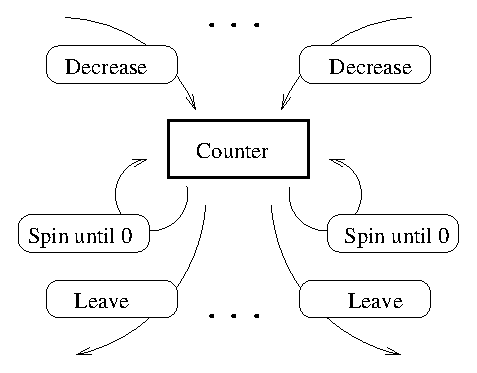
\includegraphics[angle=0, scale=.85]{fetchandadd.eps}
    \caption{Barrier implemented with fetch-and-add}
    \label{fig:fetchandadd}
  \end{center}
\end{figure*}

On a POWER4 system, the fetch-and-add operation is implemented
using a \texttt{lwarx} (load and reserve) and \texttt{stwcx} (store conditional) instruction pair. As shown in the following assembly code, the
two instructions work together to conditionally store a word to an
indexed memory position.

{\small
\begin{verbatim}
static inline int fetch_and_add (volatile int *mem, int val)
{
  int tmp, result;
  asm volatile("\n\
0:      lwarx   %0,0,%2     \n\
        add%I3  %1,%0,%3    \n\
        stwcx.  %1,0,%2     \n\
        bne-    0b          \n\
" : "=&b"(result), "=&r"(tmp) : "r" (mem), "Ir\
"(val) : "cr0", "memory");
  return result;
}
\end{verbatim}
}

The first instruction will create a reservation for use by the second
instruction. The store can only be successful when the reserved bit is
set. If not, the program will repeat the process. In this
way, the procedure prevents two threads from updating the counter at the
same time.

The advantage of this implementation is obvious. It has direct
hardware support and is quite simple in terms of coding. It does not cost
much memory either. 

As we will find out, the performance of this design is acceptable only for a
parallel system with a small number of processors, for example, less
than eight nodes.  We will see that as the number of processors increases, the
memory contention increases sharply.

\subsection{Distributed counter}
\label{sec:distcounter}

Since the fetch-and-add design has a high contention cost as the number of
processors increases, we would like to coordinate threads using multiple memory locations to reduce contention.

As a result, we produced a new implementation we call a \emph{distributed counter} shown in 
Figure \ref{fig:distcounter}. Instead of allocating one
counter in the shared memory, we allocate multiple counters as a byte
array. The size of the array is equal to the number of threads in the
barrier operation and the value of each element in the
counter is initialized to one.

\begin{figure*}[htbp]
  \begin{center}
    \includegraphics[angle=0, scale=.85]{distcounter.eps}
    \caption{Barrier implemented with distributed counter}
    \label{fig:distcounter}
  \end{center}
\end{figure*}

Similarly to the fetch-and-add barrier design, each thread arriving at the barrier
point will decrease the counter. However, unlike the fetch-and-add design, they
will decrease only their own element of the counter. In this way, there is
no need for the fetch-and-add function because simultaneous decrementing of the counter cannot happen.

In the spinning phase, each thread reads all the elements of the
distributed counter array to make sure that all of the threads have decremented
their own elements, thus arrived at the barrier point.

The idea of using different memory locations was also discussed in
\cite{Kre01}. One difference here is that in their implementation the
array element is increased by each thread continuously to mark the
``milestones'' of the synchronization.

From the test data shown later, we can see that this
barrier design outperforms the fetch-and-add design and requires only a modest increase in memory (proportional to number of threads).
With a 32-processor POWER4 system, we did not incur severe memory cost.
As in the fetch-and-add design, we can assign multiple counters for multiple
barriers, simplify the implementation.

\subsection{Distributed counter with padding}
\label{sec:distcounterpadding}

One problem with the distributed counter design as described in the
previous section is that false sharing can happen between elements of
the counter array which reside on the same cache line.  The result is that
contention happens in the memory system even though counter storage is not
strictly shared.  False
sharing can be eliminated by allocating the counter such that no two counter elements reside on the same cache line as shown in 
Figure \ref{fig:paddeddistcounter}.

\begin{figure*}[htbp]
  \begin{center}
    \includegraphics[angle=0, scale=.85]{paddeddistcounter.eps}
    \caption{Barrier implemented with padded distributed counter}
    \label{fig:paddeddistcounter}
  \end{center}
\end{figure*}

For each thread, the operation sequence is exactly the same as the
distributed counter design. The only thing different in the design is the
distributed counter itself. The data structure is padded corresponding
to the size of a cache line (128 bytes in a POWER4 system).

In section \ref{performance}, we will see that this further reduces the time
needed by a barrier operation. The drawback of this scheme is that
the memory impact will be amplified by the unused padding space. Among the 128 byte cache line, only
one byte is used.

We solve this problem by setting up two counter arrays in each
parallel region and allow all of the barriers in the same parallel region
to share these two counter sets.  This will reduce the memory consumption,
while taking full advantage of a padded distributed counter.

To reuse the same data structure,
we need to reinitialize the counter elements back to one after a
synchronization.
In case the program encounters
multiple barriers in a small period of time, like the EPCC test. We
need make sure that when we reinitialize the counter for the second
barrier, we do not contaminate the previous one.

Suppose we have a very fast and a very slow thread,
when the fast thread is free and encounters
another barrier right away, it needs to reinitialize the counter
before it can decrease the counter as designed. If this is the same
counter as the one used in the previous barrier, the slow thread may
still spin on checking whether all of the counter elements are zero. If
the bit is reinitialized to one, the slow thread will not leave the
first barrier nicely.

By having two counters, the threads can always initialize the alternative
counter while leaving the current one, knowing that no threads are
spinning on checking that one. Otherwise the current counter elements
can not be all zero.

We can further reduce the memory cost by merging the two arrays into
one position by using different bytes available in a cache line. If 
two barriers are not too close to each other, this won't affect the 
overall performance, but will halve the memory cost.

\subsection{Combined with local sensor}
\label{sec:combined}

Another interesting design was exploited in \cite{Mel91} and
\cite{Nik99}. In comparison to the fetch-and-add barrier, the
difference is that the authors did not let the threads spin on
checking the hot accessed counter, but instead used a separate local sensor.

A bit is allocated in the shared memory local to each thread, and
initialized to one before a barrier starts. Each thread, after
decreasing the counter with a fetch-and-add operation, spins on
checking the local bit. The last thread, the one that decreases the counter
to zero, will set all the sensor bits to zero, signaling the spinning threads
that they are free to leave. Thus, the counter is read many fewer times in the latter
part of the barrier synchronization.

We implemented this barrier in our test environment and the
performance data is available in the next section. 

Finally, we can combine this idea with what we have in previous
designs to create a new barrier scheme.

\begin{figure*}[htbp]
  \begin{center}
    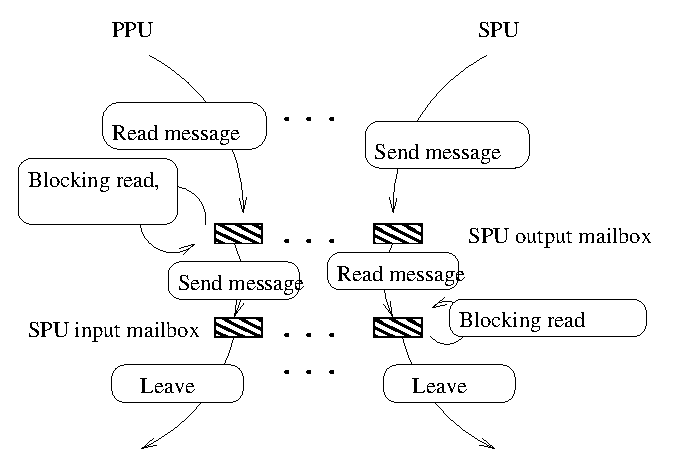
\includegraphics[angle=0, scale=.85]{combined.eps}
    \caption{Combined barrier with distributed counter and local sensor}
    \label{fig:combined}
  \end{center}
\end{figure*}

In Figure \ref{fig:combined}, we have both a padded distributed
counter and a local sensor. The local sensor is the same as the
distributed counter, implemented as an array of cache lines.

Before a barrier starts, all the elements of the counter array will be set
to one, as will the local sensor counter array. We let one thread in the group, for
instance the master thread, act as if it is the last thread. It will
decrease its own element of the distributed counter array and then spin to
check whether all of the counter elements are zero. The rest of the
threads will decrease their own counter elements and then spin on
checking their own local sensors. 

When the designated thread finds the counter elements are all zero, it will set
all the counter elements back to one and then zero all of the elements in the
local sensor array.  Finally, when all of the threads leave the barrier after
their local sensor is zeroed, they reset their local sensor back to one.

Algorithm \ref{alg:barrier} describes this more
formally\footnote{Note that we did not emphasize the data structure
  here, they can be either a padded one or not, or even share the same
  cache line as we discussed previously.}.

\begin{algorithm}[h]
  \SetLine
  \AlgData{Distributed counter with each element as one}
  \AlgData{Local sensor with each element as one}
  \BlankLine
  \Begin {
    Decrease my own distributed counter element\;
    \eIf{I am the master thread}{
      \Repeat{all distributed counter elements are zero} {
        \lForEach{element in distributed counter}{check if it is zero}
      }
      \ForEach{element in distributed counter}{set it back to one}
      \ForEach{element in local sensor}{set it to zero}
    }{
      \Repeat{it is zero} {
        check my local sensor element
      }
    }
    Set my own local sensor element back to one\;
  }
  \caption{Barrier with distributed counter and local sensor}
  \label{alg:barrier}
\end{algorithm}

We would like to avoid allocating two cache line arrays for every
barrier.  In our test code, we use the same idea to reduce memory cost
as we did for padded distributed array by letting all the barriers in
a parallel region share the same pair of counter and sensor. 

Unlike the previous situation, we do not need two groups of counter
here.  The reason is that the last thread resets the counter values
before any thread leaves the barrier, and each thread will reset its
own sensor right after it is free.

In the combined barrier case, even if the fast thread is already
spinning on checking its sensor for the second barrier, its counter
element value will not affect the slow thread. This is so because, by
the time the fast thread can decrease its counter element, the slowest
thread must have passed the phase of resetting all the counter
elements.  The counter reset operation is done by the last thread (the
slowest one) before it frees the remaining threads from the first
barrier. In the worst case, the slowest thread will still be spinning
on its sensor for the first barrier when the fast thread is spinning
on its sensor for the second barrier.

In order to save memory, we could also merge the counter and the
sensor into the same cache line using a different byte position.
However, this would increase the barrier overhead (largely nullifying
the benefit of the local sensors) as the counter and the sensor will
be accessed at the same time in the same synchronization.

